\documentclass[12pt]{article}

\usepackage{fullpage}
\usepackage{multicol,multirow}
\usepackage{tabularx}
\usepackage{graphicx}
\usepackage{ulem}
\usepackage[utf8]{inputenc}
\usepackage[russian]{babel}


\begin{document}

\section*{Лабораторная работа №\,1 по курсу дискрeтного анализа: сортировка за линейное время}

Выполнил студент МАИ группы М8О-201Б \textit{Ефимов Александр}.

\subsection*{Постановка задачи}


Требуется разработать программу, осуществляющую ввод пар «ключ-значение»,
  их упорядочивание по возрастанию ключа указанным алгоритмом сортировки за линейное время и вывод отсортированной последовательности.
  
 \ Вариант 5-1 
\begin{itemize}
\item Тип сортировки: поразрядная сортировка.
\item Тип ключа: MD5-суммы (32-разрядные шестнадцатиричные числа).
\item Тип значения: строки фиксированной длины 64 символа, во входных данных могут встретиться строки меньшей длины, при этом строка дополняется до 64-х нулевыми символами, которые не выводятся на экран.
\end{itemize}

\subsection*{Метод решения}


Сама программа состоит из трех частей:
\begin{enumerate}
\item Реализации вектора для хранения неопределенного количества данных
\item Сортировки соответствующего вектора
\item Ввода в вектор и вывода из него
\end{enumerate}
Так как работа происходит с шестнадцатиричным числами, то, для удобства, они вводятся как массивы символов, а позже переводятся в соответствующие значения в десятичной системе при помощи оперций над символами.\\
Поразраядная сортировка происходит за счет посчета количества цифр в одном и том же разряде каждого ключа за один проход и записывания их количеств в  массив чисел размером с основанием системы исчисления (например, если в втором разряде первых 5 чисел два нуля и три единицы, то в нулевую позицию массива записывается 2, во первую - 3).

После этого из нулевой позиции вычитается единица, а каждое следующее число заменяется на его сумму с предыдущим ему числом.\\
В итоге у нас получается массив, указывающий на позиции каждого ключа в отсортированном векторе

Для расстановки ключей в отсортированный вектор достаточно начать обход текущего вектора с конца до начала включительно, а ключи записывать в позицию, равную числу в ячейке массива под номером, равного цифре разряда. После записи из числа вычисть единицу.

\subsection*{Описание программы}

\begin{enumerate}
\item \textbf{Vector.h}
	\begin{itemize}
	Определяет шаблонный вектор класс
		\item Определены конструкторы для класса, а также деструктор;
		\item Swap функция для замены местами двух векторов;
		\item Перегружаны операторы приравнивания для LValue и RValue, а также оператор индексации;
		\item Методы, возвращающие указатели на начало и конец;
		\item Методы, определяющие размер вектора и его пустоту (empty).
	\end{itemize}
\item \textbf{Sort.cpp}
	\begin{itemize}
		\item Три константы показывающие на максимальные размеры строки, ключа, а также основание системы исчисления соответственно;
		\item Тип Slot, который содержит в себе ключ и соответствующую ему строку;
		\item Сама функция сортировки;
		\item \textit{int main()}.
	\end{itemize}
\end{enumerate}

\subsection*{Дневник отладки}

\begin{center}
 \begin{tabular}{| c |p{4cm}|p{5cm}|p{4cm}|} 
 \hline
 Номер & Ошибка & Обнаруженная причина &  Исправление \\
 \hline\hline
 1 & Ошибка выполнения & \textit{return 1} при пустом векторе & Заменить на \textit{return 0}  \\ 
 \hline
 2 & Неправильный ответ & Вывод текста при пустом векторе & Убрать вывод текста \\
 \hline
 3 & Превышено реальное время работы & Неверно написан шаг алгоритма сортировки & Исправление шага \\
 \hline
 4 & Ошибка выполнения & Переполнение массива посчета цифр & Изменить тип с \textit{short} на \textit{unsigned int} \\ 
 \hline
\end{tabular}
\end{center}

\subsection*{Тест производительности}

\begin{figure}[htp]

\centering
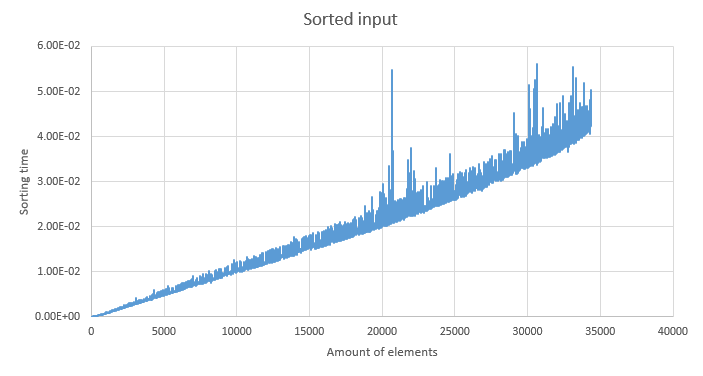
\includegraphics[width=.7\textwidth]{pics/sorted.png}\hfill
\caption{Отсортированные входящие данные}
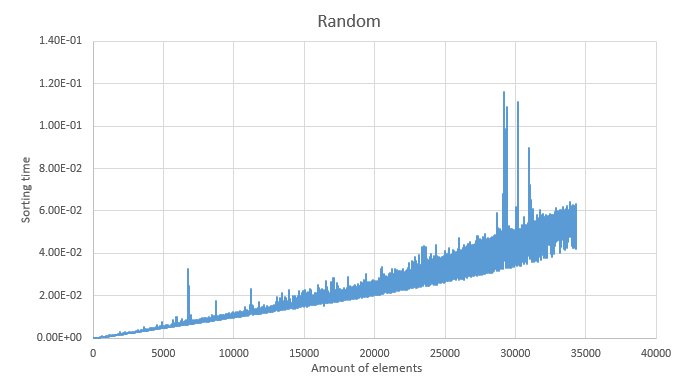
\includegraphics[width=.7\textwidth]{pics/random.png}\hfill
\caption{Случайные входящие данные}
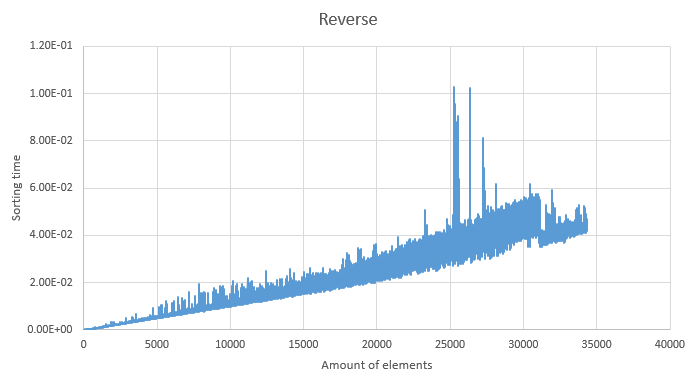
\includegraphics[width=.7\textwidth]{pics/reverse.png}
\caption{Обратно отсортированные входящие данные}
\label{fig:figure3}

\end{figure}

На рисунках 1-3 показаны разные входящие данные и времена их сортировки.
Игнорируя артефакты, вызванные особенностями работы системы, можно прийти к выводу, что данные сортируются со сравнительно одинаковой скоростью согласно сложности $O(d*(n+k))$, где $d$ -- число цифр, а $k$ -- основание системы исчисления.\\
Так как $d$ и $k$ константы, то сложность -- линейная.
\linebreak

\subsection*{Недочёты}

В связи с особенностью сортировки, а именно массива подсчета цифр, без усложнения алгоритма сортировки и/или ввода данных, количество вводимых строк ограничено размером типа этого массива (в частности, для массива типа \textit{unsigned long long} количество данных ограничено до $2^{64}$ ключей и строк).

\subsection*{Выводы}

Поразрядная сортировка может быть использована на месте сортировки подсчетом там, где диапазон вводимых данных может быть слишком большим для сортировки подсчетом. Также, поразрядная сортировка часто используется при сортировки карт и может быть использована при сортировки слов (при этом начиная с первого разряда, а не с последнего).

\end{document}
